\chapter{Uczenie na podstawie informacji obrazowej}

W poniższym rozdziale opisano podejście zastosowane w pracy \cite{mnih2015human}, które pozwoliło na skuteczną naukę na podstawie surowych danych obrazowych. Dalej przedstawiono wybrane techniki zwiększające skuteczność praktycznego uczenia ze wzmocnieniem. Na końcu opisano środowisko 3D VizDoom, oraz scenariusze na których przeprowadzono eksperymenty obliczeniowe.
\section{Uczenie na podstawie surowych danych obrazowych - Atari 2600}

Jednym z największych przełomów uczenia ze wzmocnieniem ostatnich lat była praca \break \cite{mnih2015human}, w której autorzy wykorzystali głębokie sieci neuronowe do stworzenia agenta potrafiącego grać w klasyczne gry z Atari 2600 na poziomie porównywalnym z człowiekiem, wykorzystując jako reprezentację stanu jedynie surowy zapis obrazu 2D. Dotychczas, jak w poprzednich przykładach, algorytmy uczenia ze wzmocnieniem opierały się na manualnie stworzonej reprezentacji stanów. W \cite{mnih2015human} pokazano, że możliwe jest stworzenie rozwiązania, które samo będzie potrafiło ekstrahować wysokopoziomowe cechy z niskopoziomowych danych. Zaproponowana architektura, jak również pomysłowe usprawnienia zwiększające stabilność uczenia zaproponowane w artykule, a opisane w rozdziale \ref {enhancements} stanowią obecnie podstawę i punkt odniesienia dla większości dalszych badań na temat uczenia ze wzmocnieniem.

Jako aproksymator funkcji $Q$ wykorzystano głęboką sieć neuronową. Z tego powodu opisywane podejście określa się często skrótem DQN \textit{(ang. Deep Q Network)}, czyli głęboka sieć Q. Analogicznie jak w obecnie stosowanych architekturach rozpoznawania obrazu, pierwsze warstwy sieci to warstwy konwolucyjne, które wykrywają kolejno nisko i wysokopoziomowe cechy obrazu. Dalsze warstwy, w pełni połączone, łączą informacje z warstw konwolucyjnych we wnioski na temat stanu świata, na podstawie których następne warstwy mogą określić wartość funkcji $Q$.

\subsection{Warstwy konwolucyjne}
Warstwy konwolucyjne \textit{(ang. convolutional layers)} są podstawowym elementem sieci neuronowych służących do analizy obrazów. W przeciwieństwie do warstw w pełni połączonych \textit{(ang. fully connected)}, w których każdy neuron łączy się z wyjściem każdego neuronu z warstwy poprzedniej, warstwy konwolucyjne analizują obraz z podziałem na małe, niezależne fragmenty. Warstwa konwolucyjna składa się z wielu filtrów. Każdy filtr rozpoznaje konkretny wzorzec w małym fragmencie obrazu (na przykład o wielkości 6x6 pikseli). Filtr ,,przykładany'' jest kolejno do kolejnych fragmentów obrazu (z przesunięciem równym wartości \textit{kroku}). Każdy z filtrów wykrywa jakąś cechę. W pierwszych warstwach mogą to być na przykład krawędzie, w dalszych bardziej złożone cechy. Wyjście warstwy konwolucyjnej można intuicyjnie postrzegać jako informację, gdzie na obrazie wykryto dane cechy.



\section{Q-learning - usprawnienia}\label{enhancements}
Skuteczność i stabilność Q-learningu może zostać drastycznie polepszona dzięki zastosowaniu następujących technik.

\subsection{Pamięć powtórek}\label{replaymemory}

Szkielet uczenia ze wzmocnieniem opiera się na zbieraniu doświadczeń i uaktualnianiu na ich podstawie stanu wiedzy agenta. W praktyce, doświadczenia zbierane bezpośrednio po sobie są silnie skorelowane - przykładowo agent uczący się na podstawie obrazu jazdy samochodem w kolejnych klatkach widzi niemal identyczne obrazy i wykonuje najczęściej te same akcje. Oznacza to, że aktualizowanie wiedzy agenta na podstawie nowych doświadczeń, czy to pojedynczo czy w paczkach, będzie skutkować funkcją obciążoną w kierunku tych, nowych doświadczeń.

Aby temu zapobiec w \cite{mnih2015human} zaproponowano metodę pamięci powtórek \textit{(ang. Replay memory)}. Metoda opiera się na zapamiętywaniu znacznej ilości najnowszych doświadczeń. Po każdym kroku nowe doświadczenia dodawane są do pamięci (w przypadku braku miejsca zastępując najstarsze), a następnie z pamięci wybierana jest losowa próbka doświadczeń, na podstawie których aktualizowana jest wiedza agenta. Dzięki tej technice dane użyte do nauki przez agenta są nieskorelowane i niezależne. Dodatkowo, dzięki dostępowi do starszych danych agent jest mniej podatny na obniżanie jakości gry na skutek krótkotrwałych spadków wyników.

Dalsze rozszerzenia metody mają na celu np. priorytetyzowanie używania do nauki najważniejszych doświadczeń \cite{DBLP:journals/corr/SchaulQAS15}.
\subsection{Zamrażanie docelowej sieci}\label{fixedtarget}

Podobnie jak pamięć powtórek, zamrażanie docelowej sieci \textit{(ang. Target network freezeing / fixed target network)} zostało zaproponowane w \cite{mnih2015human} i służy zmniejszeniu skutków obciążenia rozkładu danych uczących zebranych przez agenta, a wynikającego ze sposobu zbierania próbek. Zamrażanie sieci zakłada utrzymywanie dwóch funkcji Q - starej i nowej. Agent działa na podstawie nowej funkcji, ale wartości Q ,,docelowych'' stanów używanych do aktualizacji wartości Q (\ref{tdl}) pobierane są ze starej funkcji. Co jakiś czas do starej funkcji Q przepisywana jest nowa funkcja Q.

Technika ma na celu zniwelowanie oscylacji i ustabilizowanie zachowań agenta. Dzięki wykorzystaniu ,,zamrożonych'' wartości do nauki funkcji Q zerwane jest sprzężenie zwrotne pomiędzy zebranymi danymi a wartościami docelowymi.

\subsection{Kształtowanie}\label{shaping}
W wielu zadaniach stawianych przed uczeniem ze wzmocnieniem osiągnięcie celu jest bardzo trudne, a agent dostaje nagrody dopiero po osiągnięciu stanów terminalnych, albo na zaawansowanym etapie zadania. Agent uczący się na podstawie prób, błędów i losowych akcji nie jest najczęściej w stanie wykonać wystarczająco dużej części zadania, żeby dostać informację zwrotną w postaci nagrody, a więc nie ma jak się uczyć lub uczenie następuje bardzo wolno.

Kształtowanie \textit{(ang. Shaping)} (\cite{Mataric94rewardfunctions}) zakłada sztuczne wprowadzenie do środowiska dodatkowych nagród, które agent będzie dostawał po wykonaniu etapów pośrednich zadania. Przykładowo, przy grze w szachy, w której agent dostaje nagrodę tylko za wygraną lub przegraną (1 lub -1) można byłoby wprowadzić nagrodę 0.1 za zbijanie figur przeciwnika.

Kształtowanie wymaga możliwości ingerencji w środowisko albo percepcję agenta (rozpoznawanie, kiedy agent powinien dostać sztuczną nagrodę i ingerowanie w odczyty nagrody dokonywane przez agenta). Co ważniejsze, wymaga wiedzy eksperckiej na temat zadania wykonywanego przez agenta (możliwość określenia sensownych etapów zadania, na których agent miałby dostać sztuczną nagrodę) i wiedzy na temat środowiska, w którym agent się porusza (wysokość sztucznej nagrody musi być dopasowana do prawdziwych nagród, które może dostawać agent). Dodatkowo, kroki określone przez eksperta mogą wymuszać nieoptymalną politykę działania i powstrzymać agenta przed odkryciem optymalnych strategii.

\subsection{Dropout}\label{dropout}

Technika \textit{dropoutu}, opisana w pracy \cite{Srivastava:2014:DSW:2627435.2670313} jest narzędziem regularyzacji głębokich sieci neuronych i służy zapobieganiu zjawisku przeuczenia sieci.

\textit{Dropout} polega na losowym traktowaniu wybranych neuronów jak usuniętych z sieci, na czas pojedynczych iteracji uczenia. W każdej kolejnej iteracji nauki inne neurony są losowo wygaszane. Dzięki temu wiedza na temat konkretnych cech jest rozpropagowana między wieloma neuronami i nie ma nadmiernej specjalizacji neuronów. Na etapie testowania sieci żadne z neuronów nie są usuwane, a aktywacje są normalizowane, żeby sumaryczna siła aktywacji odpowiadała sumarycznej sile aktywacji neuronów podczas treningu.

W używanych narzędziach \textit{dropout} zaimplementowany jest najczęściej jako oddzielny typ warstwy sieci, przepuszczający do nastepnej warstwy tylko wybrane aktywacje neuronów z poprzedniej warstwy, a resztę aktywacji propagując jako 0.

\section{Środowisko VizDoom}

Środowisko VizDoom, przedstawione w \cite{DBLP:journals/corr/KempkaWRTJ16}, jest narzędziem do testowania algorytmów sterowania na podstawie surowych danych o obrazie 3D. Środowisko bazujące na klasycznej grze Doom, w której gracz widzi trójwymiarowy świat z perspektywy pierwszoosobowej i strzela do piekielnych potworów. W stosunku do nauki w środowisku 2D, takim jak Atari 2600 [REF], nauka w środowisku  3D jest wielkim krokiem naprzód i stanowi znacznie lepsze przybliżenie nauki w realnym świecie.

VizDoom oferuje wygodny interfejs, który doskonale wpisuje się w standardowy szkielet metod uczenia ze wzmocnieniem. VizDoom potrzebuje mało zasobów, może działać bez środowiska graficznego, jest wydajny, pozwala na uruchamianie wielu instancji równolegle oraz na wygodne tworzenie nowych scenariuszy dopasowanych do potrzeb problemów badawczych. Vizdoom udostępnia interfejs programistyczny dla Pythona, Javy, C++ i Lua. Preferowany i najbardziej rozwijany jest Python.

Przykładowe minimalne użycie środowiska VizDoom przedstawione jest poniżej (prezentowany kod jest zmodyfikowanym przykładem \textit{scenarios.py} dołączonym do środowiska):

\begin{lstlisting}[language=iPython]
from vizdoom import DoomGame

game = DoomGame()

game.load_config("../../scenarios/basic.cfg")

game.set_screen_resolution(ScreenResolution.RES_640X480)
game.set_window_visible(True)
game.init()

# Creates all possible actions depending on how many buttons there are.
actions = prepare_actions(game.get_available_buttons_size())

episodes = 10

for i in range(episodes):
    game.new_episode()
    while not game.is_episode_finished():
        # Gets the state and possibly to something with it
        state = game.get_state()
        # Makes a random action and save the reward.
        reward = game.make_action(choose(state, actions))
	new_state  = game.get_state() 
	learn(state,game.get_last_action(), reward, new_state)
\end{lstlisting}

\section{Wykorzystane scenariusze}
Eksperymenty przeprowadzono na następujących scenariuszach, reprezentujących łatwy, średni i wysoki poziom trudności. W ostatecznych porównaniach nie wykorzystano scenariusza podstawowego, ponieważ ma zbyt niski poziom skomplikowania żeby zobrazować zależności pomiędzy metodami.

\subsection{Podstawowy (ang. Basic)}\label{scenario_basic}
Środowisko składa się z prostokątnego pomieszczenia. Agent startuje w jednym końcu pomieszczenia, po środku ściany, a w losowym miejscu pod przeciwległą ścianą znajduje się pojedynczy, nieruchomy przeciwnik.

Agent może strzelać do przeciwnika oraz poruszać się w prawo lub w lewo. Agent ma ograniczoną amunicję i dostaje punkt za trafienie przeciwnika.

Racjonalna strategia polega na przesunięciu się w kierunku przeciwnika i oddaniu do niego pojedynczego strzału.


\begin{figure}[H]
	\begin{floatrow}
		\ffigbox{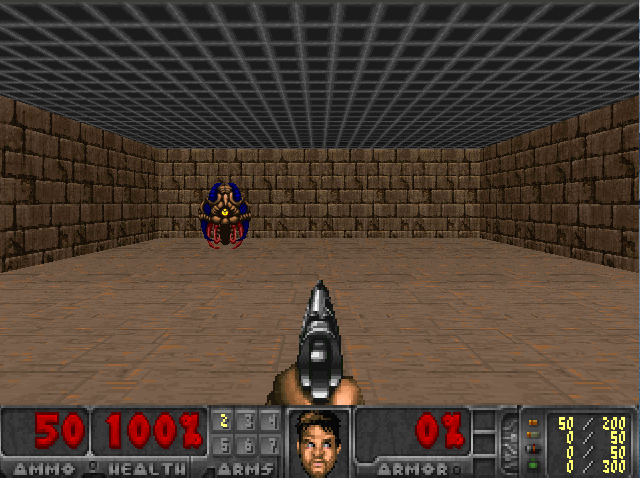
\includegraphics[scale = 0.35]{figures/screens/scenarios/basic.png}}{\caption{Scenariusz podstawowy}\label{fig:scenario_basic}}
	\end{floatrow}
\end{figure}

\subsection{Obrona środka (ang. Defend the center)}\label{scenario_dtc}
Środowisko składa się z kolistej areny. Agent znajduje się na środku areny, a na jej krańcach losowo pojawiają się przeciwnicy, którzy poruszają się w stronę agenta, a po dotarciu do niego zadają mu obrażenia. Są dwa rodzaje przeciwników różniących się wyglądem i szybkością poruszania.

Agent może strzelać i kręcić się wokół własnej osi w lewo i prawo. Agent ma ograniczoną amunicję i dostaje punkty za każde trafienie przeciwnika.

Racjonalna strategia polega na kręceniu się w jedną stronę w kółko, ignorowaniu odległych przeciwników i strzelaniu do bliskich, priorytetyzując szybszych przeciwników. Ignorowanie dalekich przeciwników jest konieczne, żeby w czasie strzelania do nich inni przeciwnicy nie zaszli agenta od tyłu - optymalna strategia wymaga zajmowania się najpierw najbliższym zagrożeniem.

\begin{figure}[H]
	\begin{floatrow}
		\ffigbox{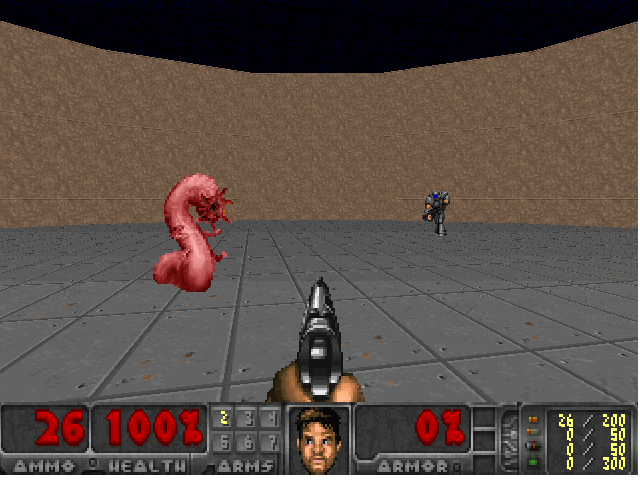
\includegraphics[scale = 0.35]{figures/screens/scenarios/dtc.png}}{\caption{Scenariusz obrona środka}\label{fig:scenario_dtc}}
	\end{floatrow}
\end{figure}


\subsection{Trudne zbieranie apteczek (ang. Health gathering supreme) }\label{scenario_hgs}
Środowisko składa się z labiryntu, którego podłoga jest pokryta kwasem. Agent startuje w losowym miejscu labiryntu. W tym scenariuszu nie ma ruchomych przeciwników. Na podłodze labiryntu pojawiają się losowo apteczki, które dodają agentowi punkty życia i miny, które zabierają agentowi punkty życia. Kwas na podłodze nieustannie odbiera agentowi punkty życia. 

Agent może poruszać się do przodu, na ukos w prawo lub w lewo oraz kręcić się wokół własnej osi w prawo lub w lewo. Agent dostaje punkty za pozostawanie przy życiu - im dłużej potrwa gra, tym większą sumę punktów zdobędzie agent.

Racjonalna strategia polega na chodzeniu po labiryncie, niewchodzeniu na miny i zbieraniu apteczek, preferując kierowanie się do dużych skupisk apteczek. Wskazane jest unikanie zbierania pojedynczych, odizolowanych apteczek, gdyż liczba punktów życia uzyskana z takiej apteczki może być mniejsza niż liczba punktów życia straconych na dotarcie do apteczki. Wskazane jest niepozostawanie w jednym obszarze labiryntu, ponieważ nowe apteczki mogą nie pojawiać się wystarczająco szybko, żeby utrzymać agenta przy życiu.

Co istotne, w tym scenariuszu bardzo często optymalna decyzja nie jest jednoznaczna - sensownie działający ekspert i agent mogą często wybierać pomiędzy wieloma poprawnymi drogami i zachowaniami.

\begin{figure}[H]
	\begin{floatrow}
		\ffigbox{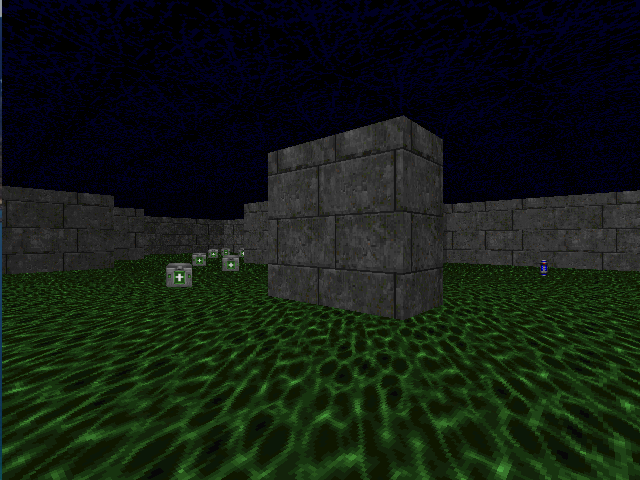
\includegraphics[scale = 0.35]{figures/screens/scenarios/hgs.png}}{\caption{scenariusz trudne zbieranie apteczek}\label{fig:scenario_hgs}}
	\end{floatrow}
\end{figure}

